% !TeX spellcheck = en_US

\chapter{Theoretical and Experimental Results}\label{chp:theoretical_and_experimental_results}
\section{Training data}
\subsection{Airtiler - A data set generation tool}
For the training, we wanted to use publicly and freely available data. Not only do high-resolution orthophotos cost a fair deal; we also wanted to ensure that other researchers would be able to replicate our study. We thus used OpenStreetMap to obtain the vector data and Microsoft Bing Maps for the imagery.

A data set consisting of satellite imagery and images of the ground truths can be created using the Python module Airtiler \cite{airtiler}. This tool was developed by the author during this master thesis. It allows for configuring one or more bounding boxes, together with several other options such as zoom level and OpenStreetMap attributes. \autoref{lst:results:airtiler_config} shows a sample configuration used by Airtiler.

\begin{minipage}{\linewidth}
\begin{lstlisting}[caption={Sample configuration for Airtiler},captionpos=b,label=lst:results:airtiler_config]
{
  "options": {
    "target_dir": "",
    "zoom_levels": [18,19],
    "separate_instances": false
  },
  "query": {
    "tags": [
    	"highway",
    	"building",
    	"leisure=swimming_pool",
    	"sport=tennis",
    	"landuse=vineyard"
    ]
  },
  "boundingboxes": {
    "giswil_1": [
    	8.1566193073,
    	46.7783248574,
    	8.1681635349,
    	46.7905387509
    ],
    "giswil_2": [
    	8.1388001434,
    	46.7778439103,
    	8.1562840923,
    	46.7880064196
    ],
    "goldach_rorschacherberg": [
    	9.440673825,
    	47.4534664711,
    	9.5168056457,
    	47.4896115582
    ]
  }
}
\end{lstlisting}
\end{minipage}

In the next step, the configured bounding boxes are iterated, and for each box, all tiles according to the tile map service (TMS) specification \cite{tmsspec} are processed. This includes the download of the corresponding orthophoto from Bing Maps and the creation of at least one binary image. The binary image contains all ground-truth instances for the current class – such as building or highway – that was specified in the configuration. This step creates one satellite image and one or more binary images per tile. If, for the current tile, no ground truths according to the configuration are found, no images for this tile are created. \autoref{fig:results:airtiler_output_description} shows the output of a single tile, generated by Airtiler. An important point is the file names. These names are generated from the content of the file, which makes the loading and interpretation of the data set rather simple. Image names include the file extension \textit{.tiff} whereas the masks have the extension \textit{.tif}.

\begin{figure}[H] 
\centering
  \begin{subfigure}[b]{0.4\linewidth}
    \centering
    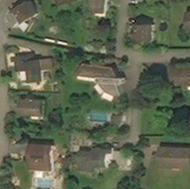
\includegraphics[width=0.9\linewidth]{chapters/theoretical_and_experimental_results/images/18_138079_170377.png}
            \caption{\detokenize{18_138079_170377.tiff}}
            \label{fig:results:airtiler_output_orthophoto}
    \vspace{4ex}
  \end{subfigure}%% 
  \begin{subfigure}[b]{0.4\linewidth}
    \centering
            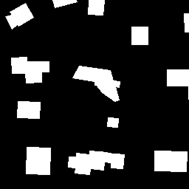
\includegraphics[width=0.9\linewidth]{chapters/theoretical_and_experimental_results/images/18_138079_170377_building.png}
            \caption{\detokenize{18_138079_170377_building.tif}}
            \label{fig:results:airtiler_output_building}
    \vspace{4ex}
  \end{subfigure} 
  \begin{subfigure}[b]{0.4\linewidth}
    \centering
            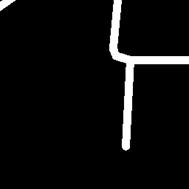
\includegraphics[width=0.9\linewidth]{chapters/theoretical_and_experimental_results/images/18_138079_170377_highway.png}
            \caption{\detokenize{18_138079_170377_highway.tif}}
            \label{fig:results:airtiler_output_highway}
  \end{subfigure}%%
  \begin{subfigure}[b]{0.4\linewidth}
    \centering
    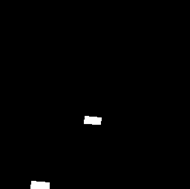
\includegraphics[width=0.9\linewidth]{chapters/theoretical_and_experimental_results/images/18_138079_170377_swimming_pool.png} 
            \caption{\detokenize{18_138079_170377_pool.tif}}
            \label{fig:results:airtiler_output_pool}
  \end{subfigure} 
  \caption{Output of Airtiler for the TMS tile (x,y)=(138079,170377) at zoom level 18.}
  \label{fig:results:airtiler_output_description}
\end{figure}

\subsection{Publicly available data sets}
Several data sets are publicly available from several source (\cite{VolodymyrMnih.2013}, \cite{spacenet}, \cite{isprs-vaihingen}, \cite{isprs-potsdam}, \cite{Helber.20170831}, \cite{deepsat}).

\section{Mapping Challenge}
At the time of writing, the platform crowdAI hosted a challenge called Mapping Challenge \cite{mappingchallenge}, which focused on detecting buildings from satellite imagery. To gain additional knowledge regarding the performance of Mask R-CNN, we decided to participate in the challenge. \autoref{tab:results:mapping_challenge_results} shows the changes made to the Mask R-CNN config and their impact on the prediction accuracy.

\newcolumntype{b}{>{\hsize=2.3\hsize}X}
\newcolumntype{s}{>{\hsize=.5\hsize}X}
\newcolumntype{m}{>{\hsize=.9\hsize}X}

\begin{table}[H]
\begin{tabularx}{\textwidth}{sssbss}
    \# Epochs & \# Steps / Epoch & \# Validation Steps & Config Change & AP@0.5 & AR@0.5 \\  \midrule
100 & 2500 & 150 & - & 0.798 & 0.566 \\ 
100 & 2500 & 150 & Image mean RGB updated & 0.799 & 0.564 \\ 
100 & 2500 & 150 & Mini mask disabled & 0.807 & 0.573 \\ 
100 & 5000 & 200 & + validation steps & 0.821 & 0.599 \\ 
100 & 10000 & 200 & + steps / epoch & 0.833 & 0.619 \\ 
100 & 20000 & 300 & + Validation steps, + steps / epoch & 0.853 & 0.885 \\  \bottomrule
\end{tabularx} 
    \caption{Mapping challenge results}
    \label{tab:results:mapping_challenge_results}
\end{table}

Generally, the results indicated that fine-tuning the hyperparameters improved the accuracy and that the impact was intensified merely through longer training. However, in longer training it must be ensured that the network does not overfit. In the case of an existing architecture, such as Mask R-CNN, this precaution has already been applied. If one develops a new architecture, overfitting must be taken care of, for example using a technique called Dropout \cite{Srivastava.2014}. Generally, Dropout randomly disables some units during the training. As a result, the model constantly changes and such change makes overfitting less likely.

\section{Microsoft COCO Annotation Format}
For the crowdAI Mapping Challenge \cite{mappingchallenge}, the instances were represented in Microsoft COCO annotation format \cite{cocoformat}. Unfortunately, using this format, it is impossible to represent polygons that have holes in them\footnote{\url{https://github.com/cocodataset/cocoapi/issues/153, 21.05.2018}}. Because there were many buildings that could require such representation, we decided not to use this format and instead used images for the representation of the ground truths.

\begin{figure}[H]
	\centering
	\begin{subfigure}{0.4\textwidth}
		\centering
    	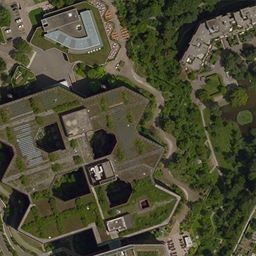
\includegraphics[width=0.9\linewidth]{chapters/theoretical_and_experimental_results/images/building_with_hole.png}		    \caption{A building with multiple holes}
	\end{subfigure}~
		\begin{subfigure}{0.4\textwidth}
		\centering
    	
\includegraphics[width=0.9\linewidth]{chapters/theoretical_and_experimental_results/images/building_with_hole_gt.png}		    \caption{Predicted building masks}
	\end{subfigure}
	\caption{The corresponding ground truth}
	\label{fig:results:buildings_with_holes_gt}
\end{figure}
